\documentclass[12pt]{article}
\usepackage[utf8]{inputenc}
\usepackage[spanish]{babel}
\usepackage{amsmath}
\usepackage{amssymb}
\usepackage{graphicx}
\usepackage{geometry}
\geometry{a4paper, margin=1in}
\usepackage{listings}
\usepackage{xcolor} % Para colores personalizados
\lstset{
    language=Python,                % Lenguaje del código
    basicstyle=\ttfamily\small,    % Estilo de fuente
    backgroundcolor=\color{gray!10}, % Fondo claro
    frame=single,                  % Borde alrededor del código
    numbers=left,                  % Números de línea
    numberstyle=\tiny,             % Estilo de los números
    keywordstyle=\color{blue},     % Color de las palabras clave
    stringstyle=\color{red},       % Color de las cadenas
    commentstyle=\color{green},    % Color de los comentarios
    breaklines=true,               % Salto de línea automático
    tabsize=4                      % Tamaño de la tabulación
}
% Paquete para manejar bibliografía
\usepackage[style=apa, backend=biber]{biblatex} % Opcionalmente, puedes usar 'style=authoryear' para estilo autor-año
\addbibresource{referencias.bib} % Nombre de tu archivo .bib


\title{Modelo Matemático para la Bioconversión de Residuos por Larvas de Mosca Soldado Negra y Producción de $CO_2$}
\author{John Leal}
\date{}

\begin{document}

\maketitle

\section{Introducción}
En este documento se presenta un modelo matemático para describir el proceso de bioconversión de residuos orgánicos mediante larvas de mosca soldado negra (\textit{Hermetia illucens}). El objetivo es determinar la cantidad de dióxido de carbono ($CO_2$) generada durante el proceso. Se realizan suposiciones simplificadoras para facilitar el análisis (\cite{shulerbioprocess2017}; \cite{dienerblack2011}).

\section{Suposiciones del Modelo}
Para modelar el proceso, se consideran las siguientes suposiciones:
\begin{itemize}
    \item La biomasa de residuos disponibles disminuye debido al consumo por parte de las larvas.
    \item El crecimiento larvario depende de la disponibilidad de residuos y sigue una cinética tipo Monod.
    \item La producción de $CO_2$ está directamente relacionada con el consumo de residuos.
    \item Los residuos se convierten en biomasa larvaria y $CO_2$ con rendimientos específicos.
    \item Las condiciones ambientales (temperatura, pH, etc.) son óptimas y constantes.
\end{itemize}

\section{Variables y Parámetros}
Definimos las siguientes variables y parámetros clave del modelo:

\begin{itemize}
    \item $B(t)$: Biomasa de residuos disponibles en el tiempo $t$ [g]. \\
    Representa la cantidad de residuos orgánicos presentes en el sistema en un instante dado. Esta biomasa disminuye con el tiempo debido al consumo por parte de las larvas de mosca soldado negra. La dinámica de $B(t)$ está descrita por la ecuación diferencial que modela el consumo de residuos siguiendo una cinética tipo Monod.

    \item $L(t)$: Biomasa total de larvas en el tiempo $t$ [g]. \\
    Indica la masa total de las larvas presentes en el sistema en un instante dado. El crecimiento de las larvas depende de la disponibilidad de residuos y está limitado por factores como el espacio físico y la capacidad del sistema para sostener una población máxima de larvas ($L_{\text{max}}$).

    \item $C(t)$: Cantidad acumulada de $CO_2$ producida en el tiempo $t$ [g]. \\
    Representa la cantidad total de dióxido de carbono liberado durante el proceso de bioconversión. Este subproducto es generado por el metabolismo respiratorio de las larvas al consumir los residuos orgánicos. La producción de $CO_2$ está directamente relacionada con la tasa de consumo de residuos.

    \item $\mu_L$: Tasa máxima específica de consumo de residuos por unidad de biomasa larvaria [g residuo / g larva / día]. \\
    Es un parámetro clave que describe la eficiencia con la que las larvas consumen los residuos disponibles. Este valor representa la tasa máxima a la cual las larvas pueden consumir residuos cuando estos están en exceso.

    \item $K_B$: Constante de saturación de residuos [g]. \\
    Representa la concentración de residuos a la cual la tasa de consumo es la mitad de $\mu_L$. Este parámetro refleja la afinidad de las larvas por los residuos: valores bajos de $K_B$ indican una alta afinidad (las larvas consumen eficientemente incluso cuando hay pocos residuos), mientras que valores altos indican una menor afinidad.

    \item $Y_{L/B}$: Rendimiento de biomasa larvaria por unidad de residuo consumido [g larva / g residuo]. \\
    Este parámetro indica qué fracción de la biomasa de residuos consumidos se convierte en biomasa larvaria. Depende de la eficiencia metabólica de las larvas y puede variar según el tipo de residuos y las condiciones ambientales.

    \item $Y_{C/B}$: Rendimiento de $CO_2$ por unidad de residuo consumido [g $CO_2$ / g residuo]. \\
    Representa la cantidad de dióxido de carbono generada por cada gramo de residuo consumido. Este valor está determinado por la estequiometría del metabolismo larvario y es crucial para evaluar el impacto ambiental del proceso.

    \item $L_{\text{max}}$: Biomasa larvaria máxima sostenible en el sistema [g]. \\
    Es la capacidad máxima del sistema para sostener biomasa larvaria. Este límite puede estar determinado por factores como el espacio físico, la disponibilidad de nutrientes o la competencia entre larvas. Cuando $L(t)$ alcanza $L_{\text{max}}$, el crecimiento larvario se detiene.
\end{itemize}

\section{Ecuaciones Diferenciales del Modelo}
El proceso se describe mediante el siguiente sistema de ecuaciones diferenciales:

\subsection{Consumo de Residuos}
La tasa de consumo de residuos sigue una cinética tipo Monod:
\begin{equation}
    \frac{dB}{dt} = -\mu_L \cdot \frac{B(t)}{K_B + B(t)} \cdot L(t)
\end{equation}


La tasa de consumo de residuos sigue una \textbf{cinética tipo Monod}, que es un modelo ampliamente utilizado en biología y bioingeniería para describir procesos en los que la velocidad de una reacción depende de la concentración de un sustrato limitante. En este caso, el sustrato limitante son los residuos orgánicos ($B(t)$) consumidos por las larvas de mosca soldado negra. La ecuación que describe esta cinética es:

\begin{equation}
    \frac{dB}{dt} = -\mu_L \cdot \frac{B(t)}{K_B + B(t)} \cdot L(t)
\end{equation}

A continuación, desglosamos cada componente de la ecuación y su significado:

\begin{itemize}
    \item $\frac{dB}{dt}$: Representa la \textbf{tasa de cambio de la biomasa de residuos disponibles} con respecto al tiempo [g/día]. El signo negativo indica que la cantidad de residuos disminuye con el tiempo debido al consumo por parte de las larvas.

    \item $\mu_L$: Es la \textbf{tasa máxima específica de consumo de residuos} por unidad de biomasa larvaria [g residuo / g larva / día]. Este parámetro refleja la eficiencia máxima con la que las larvas pueden consumir residuos cuando estos están en abundancia. Es una propiedad intrínseca de las larvas y puede variar según la especie y las condiciones ambientales.

    \item $B(t)$: Es la \textbf{biomasa de residuos disponibles} en el tiempo $t$ [g]. A medida que las larvas consumen los residuos, $B(t)$ disminuye.

    \item $K_B$: Es la \textbf{constante de saturación de residuos} [g]. Este parámetro representa la concentración de residuos a la cual la tasa de consumo es la mitad de $\mu_L$. En otras palabras, $K_B$ refleja la afinidad de las larvas por los residuos:
    \begin{itemize}
        \item Si $B(t) \ll K_B$, la tasa de consumo es aproximadamente lineal con respecto a $B(t)$.
        \item Si $B(t) \gg K_B$, la tasa de consumo se satura y tiende a su valor máximo ($\mu_L$).
    \end{itemize}

    \item $L(t)$: Es la \textbf{biomasa total de larvas} en el tiempo $t$ [g]. Este término refleja que el consumo de residuos es proporcional a la cantidad de larvas presentes en el sistema. Cuantas más larvas haya, mayor será la tasa de consumo.

    \item $\frac{B(t)}{K_B + B(t)}$: Este término describe la \textbf{dependencia no lineal} del consumo de residuos con respecto a la disponibilidad de residuos. Es característico de la cinética tipo Monod y tiene las siguientes propiedades:
    \begin{itemize}
        \item Cuando $B(t)$ es pequeño ($B(t) \ll K_B$), el término se comporta de manera aproximadamente lineal: $\frac{B(t)}{K_B + B(t)} \approx \frac{B(t)}{K_B}$.
        \item Cuando $B(t)$ es grande ($B(t) \gg K_B$), el término se satura y tiende a 1: $\frac{B(t)}{K_B + B(t)} \approx 1$.
    \end{itemize}
    Esto refleja que las larvas consumen residuos más rápidamente cuando hay abundancia, pero su tasa de consumo disminuye cuando los residuos escasean.

    \item $-\mu_L \cdot \frac{B(t)}{K_B + B(t)} \cdot L(t)$: Finalmente, el producto de estos términos da la \textbf{tasa neta de consumo de residuos}. La inclusión de $L(t)$ asegura que el consumo sea proporcional a la biomasa larvaria presente en el sistema.
\end{itemize}

\textbf{Interpretación Biológica}
Esta ecuación captura la dinámica del proceso de bioconversión:
\begin{itemize}
    \item En las primeras etapas del proceso, cuando hay abundancia de residuos ($B(t) \gg K_B$), el consumo es máximo y está limitado principalmente por la cantidad de larvas presentes ($L(t)$).
    \item A medida que los residuos se agotan ($B(t) \to 0$), la tasa de consumo disminuye, lo que refleja que las larvas tienen menos sustrato disponible para alimentarse.
\end{itemize}

\textbf{Importancia del Modelo}
El uso de la cinética tipo Monod permite modelar de manera realista cómo las larvas interactúan con los residuos en un sistema de bioconversión. Este modelo es útil para:
\begin{itemize}
    \item Predecir la evolución temporal de la biomasa de residuos ($B(t)$).
    \item Optimizar la cantidad inicial de residuos y larvas para maximizar la eficiencia del proceso.
    \item Evaluar el impacto de factores como la disponibilidad de residuos ($K_B$) y la eficiencia de consumo ($\mu_L$) en la dinámica del sistema.
\end{itemize}

\subsection{Crecimiento Larvario}
La biomasa larvaria aumenta proporcionalmente al consumo de residuos, pero está limitada por un factor logístico:
\begin{equation}
    \frac{dL}{dt} = Y_{L/B} \cdot \mu_L \cdot \frac{B(t)}{K_B + B(t)} \cdot L(t) \cdot \left(1 - \frac{L(t)}{L_{\text{max}}}\right)
\end{equation}

Esta ecuación describe cómo la biomasa larvaria aumenta con el tiempo debido al consumo de residuos, pero está limitada por factores como la disponibilidad de recursos y la capacidad máxima del sistema. A continuación, desglosamos cada componente de la ecuación y su significado:

\begin{itemize}
    \item $\frac{dL}{dt}$: Representa la \textbf{tasa de cambio de la biomasa larvaria} con respecto al tiempo [g/día]. Este término indica cuánto crece (o decrece) la población de larvas en función de los residuos disponibles y otros factores limitantes.

    \item $Y_{L/B}$: Es el \textbf{rendimiento de biomasa larvaria por unidad de residuo consumido} [g larva / g residuo]. Este parámetro refleja qué fracción de los residuos consumidos se convierte en biomasa larvaria. Depende de la eficiencia metabólica de las larvas y puede variar según el tipo de residuos y las condiciones ambientales.

    \item $\mu_L$: Es la \textbf{tasa máxima específica de consumo de residuos} por unidad de biomasa larvaria [g residuo / g larva / día]. Este valor representa la eficiencia máxima con la que las larvas pueden consumir residuos cuando estos están en abundancia.

    \item $\frac{B(t)}{K_B + B(t)}$: Este término describe la \textbf{cinética tipo Monod} para el consumo de residuos. Refleja cómo la tasa de consumo depende de la disponibilidad de residuos:
    \begin{itemize}
        \item Cuando $B(t)$ es pequeño ($B(t) \ll K_B$), el consumo es aproximadamente lineal con respecto a $B(t)$.
        \item Cuando $B(t)$ es grande ($B(t) \gg K_B$), el consumo se satura y tiende a su valor máximo ($\mu_L$).
    \end{itemize}
    Esto asegura que el crecimiento larvario esté directamente relacionado con la cantidad de residuos disponibles.

    \item $L(t)$: Es la \textbf{biomasa total de larvas} en el tiempo $t$ [g]. Este término refleja que el crecimiento larvario es proporcional a la cantidad de larvas presentes en el sistema. Cuantas más larvas haya, mayor será la tasa de crecimiento (hasta cierto límite).

    \item $\left(1 - \frac{L(t)}{L_{\text{max}}}\right)$: Este término representa un \textbf{factor logístico} que limita el crecimiento larvario. Aquí:
    \begin{itemize}
        \item $L_{\text{max}}$: Es la \textbf{biomasa larvaria máxima sostenible} en el sistema [g]. Representa la capacidad máxima del sistema para sostener biomasa larvaria, determinada por factores como el espacio físico, la disponibilidad de nutrientes o la competencia entre larvas.
        \item El factor logístico asegura que el crecimiento larvario disminuya a medida que $L(t)$ se acerca a $L_{\text{max}}$. Cuando $L(t) = L_{\text{max}}$, el crecimiento se detiene completamente ($\frac{dL}{dt} = 0$).
    \end{itemize}

    \item $Y_{L/B} \cdot \mu_L \cdot \frac{B(t)}{K_B + B(t)} \cdot L(t)$: Este producto describe la \textbf{tasa de crecimiento larvario sin considerar la limitación logística}. Combina la eficiencia de conversión de residuos en biomasa larvaria ($Y_{L/B}$), la cinética de consumo de residuos ($\mu_L \cdot \frac{B(t)}{K_B + B(t)}$) y la biomasa larvaria presente ($L(t)$).

    \item Multiplicando todo por $\left(1 - \frac{L(t)}{L_{\text{max}}}\right)$: Finalmente, este término ajusta la tasa de crecimiento para incluir la limitación logística. Refleja que el crecimiento larvario no puede continuar indefinidamente y se ralentiza a medida que se alcanza la capacidad máxima del sistema.
\end{itemize}

\textbf{Interpretación Biológica}
Esta ecuación captura la dinámica del crecimiento larvario en un sistema de bioconversión:
\begin{itemize}
    \item En las primeras etapas del proceso, cuando hay abundancia de residuos ($B(t) \gg K_B$) y poca competencia ($L(t) \ll L_{\text{max}}$), el crecimiento larvario es rápido y está limitado principalmente por la disponibilidad de residuos.
    \item A medida que los residuos se agotan ($B(t) \to 0$) o la biomasa larvaria se acerca a su capacidad máxima ($L(t) \to L_{\text{max}}$), el crecimiento larvario disminuye y eventualmente se detiene.
\end{itemize}

\textbf{Importancia del Modelo}
El uso de un modelo logístico combinado con la cinética tipo Monod permite describir de manera realista cómo las larvas interactúan con los residuos y cómo su crecimiento está limitado por factores biológicos y ambientales. Este modelo es útil para:
\begin{itemize}
    \item Predecir la evolución temporal de la biomasa larvaria ($L(t)$).
    \item Optimizar la cantidad inicial de residuos y larvas para maximizar la producción de biomasa larvaria.
    \item Evaluar el impacto de factores como la capacidad máxima del sistema ($L_{\text{max}}$) y la eficiencia de conversión ($Y_{L/B}$) en la dinámica del sistema.
\end{itemize}

\section{Análisis de la Producción de $CO_2$}

La producción de dióxido de carbono ($CO_2$) está directamente relacionada con el consumo de residuos por parte de las larvas de mosca soldado negra. La dinámica de esta producción se describe mediante la siguiente ecuación diferencial:

\begin{equation}
    \frac{dC}{dt} = Y_{C/B} \cdot \mu_L \cdot \frac{B(t)}{K_B + B(t)} \cdot L(t)
\end{equation}

A continuación, analizamos cada componente de la ecuación y su significado:

\begin{itemize}
    \item $\frac{dC}{dt}$: Representa la \textbf{tasa de cambio de la cantidad acumulada de $CO_2$} con respecto al tiempo [g/día]. Este término indica cuánto $CO_2$ se libera durante el proceso de bioconversión debido al metabolismo respiratorio de las larvas.

    \item $Y_{C/B}$: Es el \textbf{rendimiento de $CO_2$ por unidad de residuo consumido} [g $CO_2$ / g residuo]. Este parámetro refleja qué fracción de los residuos consumidos se convierte en $CO_2$. Depende de la estequiometría del metabolismo larvario y puede variar según el tipo de residuos y las condiciones ambientales.

    \item $\mu_L$: Es la \textbf{tasa máxima específica de consumo de residuos} por unidad de biomasa larvaria [g residuo / g larva / día]. Este valor representa la eficiencia máxima con la que las larvas pueden consumir residuos cuando estos están en abundancia.

    \item $\frac{B(t)}{K_B + B(t)}$: Este término describe la \textbf{cinética tipo Monod} para el consumo de residuos. Refleja cómo la tasa de consumo depende de la disponibilidad de residuos:
    \begin{itemize}
        \item Cuando $B(t)$ es pequeño ($B(t) \ll K_B$), el consumo es aproximadamente lineal con respecto a $B(t)$.
        \item Cuando $B(t)$ es grande ($B(t) \gg K_B$), el consumo se satura y tiende a su valor máximo ($\mu_L$).
    \end{itemize}
    Esto asegura que la producción de $CO_2$ esté directamente relacionada con la cantidad de residuos disponibles.

    \item $L(t)$: Es la \textbf{biomasa total de larvas} en el tiempo $t$ [g]. Este término refleja que la producción de $CO_2$ es proporcional a la cantidad de larvas presentes en el sistema. Cuantas más larvas haya, mayor será la tasa de producción de $CO_2$.

    \item $Y_{C/B} \cdot \mu_L \cdot \frac{B(t)}{K_B + B(t)} \cdot L(t)$: Este producto describe la \textbf{tasa neta de producción de $CO_2$}. Combina la eficiencia de conversión de residuos en $CO_2$ ($Y_{C/B}$), la cinética de consumo de residuos ($\mu_L \cdot \frac{B(t)}{K_B + B(t)}$) y la biomasa larvaria presente ($L(t)$).
\end{itemize}

\textbf{Interpretación Biológica}
Esta ecuación captura la relación entre el consumo de residuos y la producción de $CO_2$:
\begin{itemize}
    \item En las primeras etapas del proceso, cuando hay abundancia de residuos ($B(t) \gg K_B$) y una población creciente de larvas ($L(t)$), la producción de $CO_2$ es alta.
    \item A medida que los residuos se agotan ($B(t) \to 0$) o la biomasa larvaria deja de crecer ($L(t)$ se estabiliza), la producción de $CO_2$ disminuye.
\end{itemize}

\textbf{Importancia del Modelo}
El uso de esta ecuación permite predecir la cantidad total de $CO_2$ generada durante el proceso de bioconversión. Esto es crucial para:
\begin{itemize}
    \item Evaluar el impacto ambiental del proceso, especialmente en términos de emisiones de gases de efecto invernadero.
    \item Optimizar el diseño del sistema para minimizar la producción de $CO_2$ mientras se maximiza la eficiencia de bioconversión.
\end{itemize}

\section{Condiciones Iniciales}

Las condiciones iniciales son fundamentales para resolver el sistema de ecuaciones diferenciales y determinar la evolución temporal de las variables. Suponemos las siguientes condiciones iniciales:

\begin{itemize}
    \item $B(0) = B_0$: Biomasa inicial de residuos [g]. \\
    Representa la cantidad de residuos orgánicos disponibles al inicio del proceso. Este valor influye directamente en la duración del proceso y en la cantidad total de $CO_2$ producida.

    \item $L(0) = L_0$: Biomasa inicial de larvas [g]. \\
    Indica la masa inicial de larvas presentes en el sistema. Este valor afecta la velocidad inicial de consumo de residuos y la producción de $CO_2$.

    \item $C(0) = 0$: Sin $CO_2$ inicial. \\
    Suponemos que no hay $CO_2$ acumulado al inicio del proceso, ya que la producción comienza cuando las larvas empiezan a consumir los residuos.
\end{itemize}

\textbf{Impacto de las Condiciones Iniciales}
Las condiciones iniciales juegan un papel clave en la dinámica del sistema:
\begin{itemize}
    \item Un valor alto de $B_0$ (mucha biomasa de residuos) prolonga el proceso y aumenta la cantidad total de $CO_2$ producida.
    \item Un valor alto de $L_0$ (muchas larvas iniciales) acelera el consumo de residuos y la producción inicial de $CO_2$, pero también puede llevar rápidamente al agotamiento de los residuos.
    \item El valor de $C(0) = 0$ asegura que el modelo parta de un estado "limpio" sin acumulación previa de $CO_2$.
\end{itemize}

\section{Estimación de Variables y Parámetros en el Laboratorio}

Para estimar las variables y parámetros del modelo en un entorno de laboratorio, utilizaremos una canastilla de dimensiones aproximadas $160 \, \text{cm} \times 60 \, \text{cm} \times 30 \, \text{cm}$, llena de biomasa inicial ($B_0$). A continuación, describimos los procedimientos experimentales para medir o calcular cada variable y parámetro:

\subsection{Estimación de la Biomasa Inicial de Residuos ($B_0$)}
- Procedimiento: Pese la cantidad total de residuos orgánicos colocados en la canastilla antes de introducir las larvas.
- Unidades: Gramos [g].
- Consideraciones:
  - Asegúrese de homogeneizar los residuos (por ejemplo, triturándolos) para garantizar una distribución uniforme.
  - Registre la humedad de los residuos, ya que puede afectar el consumo por parte de las larvas.

\subsection{Estimación de la Biomasa Inicial de Larvas ($L_0$)}
- Procedimiento: Pese la masa total de larvas introducidas en la canastilla al inicio del experimento.
- Unidades: Gramos [g].
- Consideraciones:
  - Utilice larvas de tamaño y edad similares para asegurar consistencia en el crecimiento y el consumo.
  - Registre el número inicial de larvas para calcular la densidad larvaria por unidad de volumen.

\subsection{Medición de la Tasa Máxima Específica de Consumo de Residuos ($\mu_L$)}
- Procedimiento:
  1. Monitoree diariamente la disminución de la biomasa de residuos ($B(t)$) durante las primeras etapas del proceso, cuando los residuos están en abundancia ($B(t) \gg K_B$).
  2. Calcule $\mu_L$ como la pendiente máxima de la tasa de consumo de residuos por unidad de biomasa larvaria.
- Fórmula:
  \[
  \mu_L = \frac{\Delta B}{\Delta t \cdot L(t)}
  \]
- Unidades: Gramos de residuo / gramo de larva / día [g residuo / g larva / día].
- Consideraciones:
  - Realice mediciones repetidas para minimizar errores experimentales.
  - Asegúrese de mantener condiciones controladas de temperatura y humedad.
\subsection{Estimación de la Tasa Máxima Específica de Consumo de Residuos ($\mu_L$)}

La tasa máxima específica de consumo de residuos ($\mu_L$) es un parámetro clave que describe la eficiencia con la que las larvas consumen los residuos disponibles. A continuación, se describe un procedimiento detallado para medir y calcular $\mu_L$:

\subsubsection{Procedimiento Detallado}

1. Preparación inicial del sistema experimental:
   - Llene la canastilla con una cantidad conocida de residuos orgánicos homogeneizados ($B_0$).
   - Introduzca una población inicial de larvas de tamaño y edad similares, cuya masa total sea $L_0$.
   - Registre las condiciones ambientales iniciales (temperatura, humedad, pH) para asegurar consistencia durante el experimento.

2. Monitoreo diario de la biomasa de residuos ($B(t)$):
   - Pese diariamente los residuos restantes en la canastilla para determinar la cantidad de residuos consumidos.
   - Para pesar los residuos, retire cuidadosamente las larvas y pese solo los residuos remanentes. Luego, reintroduzca las larvas al sistema.
   - Registre la biomasa de residuos ($B(t)$) en intervalos regulares (por ejemplo, cada 24 horas) durante las primeras etapas del proceso, cuando los residuos están en abundancia ($B(t) \gg K_B$).

3. Cálculo de la tasa de consumo de residuos ($\frac{\Delta B}{\Delta t}$):
   - Calcule la disminución diaria de la biomasa de residuos ($\Delta B$) como:
     \[
     \Delta B = B(t_{\text{inicial}}) - B(t_{\text{final}})
     \]
   - Determine el intervalo de tiempo correspondiente ($\Delta t$) en días.
   - Repita este cálculo para varios días consecutivos para obtener múltiples valores de $\frac{\Delta B}{\Delta t}$.

4. Normalización por biomasa larvaria ($L(t)$):
   - Divida la tasa de consumo de residuos ($\frac{\Delta B}{\Delta t}$) por la biomasa larvaria presente en el sistema ($L(t)$) en cada intervalo de tiempo:
     \[
     \text{Tasa normalizada} = \frac{\Delta B}{\Delta t \cdot L(t)}
     \]
   - Asegúrese de medir $L(t)$ regularmente, ya que la biomasa larvaria puede aumentar con el tiempo debido al crecimiento.

5. Determinación de $\mu_L$:
   - Grafique la tasa normalizada de consumo de residuos ($\frac{\Delta B}{\Delta t \cdot L(t)}$) en función del tiempo.
   - Identifique el valor máximo de esta tasa durante las primeras etapas del proceso, cuando los residuos están en abundancia ($B(t) \gg K_B$). Este valor corresponde a $\mu_L$.
   - Si los datos son ruidosos, ajuste una curva suave o calcule el promedio de los valores máximos obtenidos.

6. Repeticiones y análisis estadístico:
   - Realice el experimento al menos tres veces con diferentes lotes de larvas y residuos para garantizar la reproducibilidad.
   - Calcule el valor promedio de $\mu_L$ y su desviación estándar para evaluar la variabilidad entre repeticiones.

\subsubsection{Consideraciones Prácticas}

- Homogeneización de residuos: Triture los residuos orgánicos antes de introducirlos en la canastilla para asegurar una distribución uniforme y facilitar el acceso de las larvas.
- Control de condiciones ambientales:
  - Mantenga una temperatura constante (por ejemplo, $25^\circ \text{C}$) y una humedad relativa óptima (por ejemplo, $60\%$).
  - Evite la acumulación de productos metabólicos (como amoníaco) que puedan inhibir el consumo de residuos.
- Manejo de larvas:
  - Use guantes limpios y herramientas esterilizadas para manipular las larvas y evitar contaminación.
  - Asegúrese de que las larvas estén bien alimentadas durante todo el experimento para maximizar su actividad.
- Corrección por mortalidad larvaria:
  - Si algunas larvas mueren durante el experimento, cuéntelas y descuente su masa del cálculo de $L(t)$.

\subsubsection{Ejemplo Numérico}

Supongamos los siguientes datos experimentales:
- Día 1: $B(t_{\text{inicial}}) = 500 \, \text{g}$, $B(t_{\text{final}}) = 480 \, \text{g}$, $L(t) = 10 \, \text{g}$,
- Día 2: $B(t_{\text{inicial}}) = 480 \, \text{g}$, $B(t_{\text{final}}) = 460 \, \text{g}$, $L(t) = 11 \, \text{g}$.

Para el Día 1:
\[
\frac{\Delta B}{\Delta t \cdot L(t)} = \frac{500 - 480}{1 \cdot 10} = \frac{20}{10} = 2.0 \, \text{g residuo / g larva / día}.
\]

Para el Día 2:
\[
\frac{\Delta B}{\Delta t \cdot L(t)} = \frac{480 - 460}{1 \cdot 11} = \frac{20}{11} \approx 1.82 \, \text{g residuo / g larva / día}.
\]

El valor máximo de estas tasas ($\mu_L$) es $2.0 \, \text{g residuo / g larva / día}$.

\section{Determinación de la Constante de Saturación de Residuos ($K_B$)}
- Procedimiento:
  1. Grafique la tasa de consumo de residuos ($\frac{dB}{dt}$) en función de la concentración de residuos ($B(t)$).
  2. Ajuste los datos a la ecuación tipo Monod:
     \[
     \frac{dB}{dt} = -\mu_L \cdot \frac{B(t)}{K_B + B(t)} \cdot L(t)
     \]
  3. Determine $K_B$ como la concentración de residuos a la cual la tasa de consumo es la mitad de $\mu_L$.
- Unidades: Gramos [g].
- Consideraciones:
  - Use software de ajuste de curvas (como Python, MATLAB o Excel) para obtener $K_B$ con precisión.
\subsection{Determinación de la Constante de Saturación de Residuos ($K_B$)}

La constante de saturación de residuos ($K_B$) es un parámetro clave que describe la afinidad de las larvas por los residuos. Representa la concentración de residuos a la cual la tasa de consumo es la mitad de la tasa máxima ($\mu_L$). A continuación, se describe un procedimiento detallado para medir y calcular $K_B$:

\subsubsection{Procedimiento Detallado}

1. Preparación inicial del sistema experimental:
   - Llene la canastilla con una cantidad conocida de residuos orgánicos homogeneizados ($B_0$).
   - Introduzca una población inicial de larvas de tamaño y edad similares, cuya masa total sea $L_0$.
   - Registre las condiciones ambientales iniciales (temperatura, humedad, pH) para asegurar consistencia durante el experimento.

2. Monitoreo de la biomasa de residuos ($B(t)$):
   - Pese diariamente los residuos restantes en la canastilla para determinar la cantidad de residuos consumidos.
   - Para pesar los residuos, retire cuidadosamente las larvas y pese solo los residuos remanentes. Luego, reintroduzca las larvas al sistema.
   - Registre la biomasa de residuos ($B(t)$) en intervalos regulares (por ejemplo, cada 24 horas).

3. Cálculo de la tasa de consumo de residuos ($\frac{dB}{dt}$):
   - Calcule la disminución diaria de la biomasa de residuos ($\Delta B$) como:
     \[
     \Delta B = B(t_{\text{inicial}}) - B(t_{\text{final}})
     \]
   - Determine el intervalo de tiempo correspondiente ($\Delta t$) en días.
   - Calcule la tasa de consumo de residuos ($\frac{dB}{dt}$) como:
     \[
     \frac{dB}{dt} = \frac{\Delta B}{\Delta t}
     \]

4. Graficación de la tasa de consumo en función de la concentración de residuos:
   - Grafique la tasa de consumo de residuos ($\frac{dB}{dt}$) en el eje vertical ($y$) en función de la concentración de residuos ($B(t)$) en el eje horizontal ($x$).
   - Asegúrese de incluir suficientes puntos experimentales para capturar la relación no lineal entre $\frac{dB}{dt}$ y $B(t)$.

5. Ajuste de los datos a la ecuación tipo Monod:
   - Utilice software de ajuste de curvas (como Python, MATLAB o Excel) para ajustar los datos experimentales a la ecuación tipo Monod:
     \[
     \frac{dB}{dt} = -\mu_L \cdot \frac{B(t)}{K_B + B(t)} \cdot L(t)
     \]
   - Normalice los datos dividiendo $\frac{dB}{dt}$ por $L(t)$ (biomasa larvaria presente en cada intervalo de tiempo) para simplificar el ajuste.
   - Ajuste los parámetros $\mu_L$ y $K_B$ utilizando métodos de mínimos cuadrados o herramientas específicas del software.

6. Determinación de $K_B$:
   - Una vez ajustada la curva, identifique el valor de $K_B$ directamente del ajuste.
   - Alternativamente, determine $K_B$ como la concentración de residuos ($B(t)$) a la cual la tasa de consumo ($\frac{dB}{dt}$) es la mitad de la tasa máxima ($\mu_L$):
     \[
     \frac{dB}{dt} = \frac{\mu_L}{2} \implies K_B = B(t) \text{ cuando } \frac{dB}{dt} = \frac{\mu_L}{2}.
     \]

7. Repeticiones y análisis estadístico:
   - Realice el experimento al menos tres veces con diferentes lotes de larvas y residuos para garantizar la reproducibilidad.
   - Calcule el valor promedio de $K_B$ y su desviación estándar para evaluar la variabilidad entre repeticiones.

\subsubsection{Consideraciones Prácticas}

- Homogeneización de residuos: Triture los residuos orgánicos antes de introducirlos en la canastilla para asegurar una distribución uniforme y facilitar el acceso de las larvas.
- Control de condiciones ambientales:
  - Mantenga una temperatura constante (por ejemplo, $25^\circ \text{C}$) y una humedad relativa óptima (por ejemplo, $60\%$).
  - Evite la acumulación de productos metabólicos (como amoníaco) que puedan inhibir el consumo de residuos.
- Uso de software de ajuste de curvas:
  - En Python, utilice bibliotecas como scipy.optimize.curve\_fit para ajustar los datos a la ecuación tipo Monod.
  - En MATLAB, use funciones como `fit` o ''lsqcurvefit''.
  - En Excel, utilice la herramienta "Solver" o gráficos de dispersión con líneas de tendencia personalizadas.
- Validación de resultados:
  - Compare los valores obtenidos de $K_B$ con datos reportados en la literatura para sistemas similares.
  - Si los valores son significativamente diferentes, revise posibles errores en el diseño experimental o en las mediciones.

\subsubsection{Ejemplo Numérico}

Supongamos los siguientes datos experimentales:
- Tasa de consumo de residuos ($\frac{dB}{dt}$) normalizada por $L(t)$:
  - $B(t) = 10 \, \text{g}, \frac{dB}{dt} = 0.5 \, \text{g/día}$,
  - $B(t) = 20 \, \text{g}, \frac{dB}{dt} = 0.8 \, \text{g/día}$,
  - $B(t) = 50 \, \text{g}, \frac{dB}{dt} = 1.0 \, \text{g/día}$ (tasa máxima, $\mu_L = 1.0 \, \text{g/día}$).

Ajustando estos datos a la ecuación tipo Monod, se obtiene:
\[
K_B = 20 \, \text{g}.
\]

Este resultado indica que la tasa de consumo de residuos alcanza la mitad de su valor máximo cuando la concentración de residuos es $20 \, \text{g}$.

\section{Cálculo del Rendimiento de Biomasa Larvaria ($Y_{L/B}$)}
- Procedimiento:
  1. Mida la biomasa larvaria final ($L_f$) al final del experimento.
  2. Calcule $Y_{L/B}$ como la relación entre el incremento en biomasa larvaria y la cantidad de residuos consumidos:
     \[
     Y_{L/B} = \frac{L_f - L_0}{B_0 - B_f}
     \]
- Unidades: Gramos de larva / gramos de residuo [g larva / g residuo].
- Consideraciones:
  - Asegúrese de secar las larvas antes de pesarlas para eliminar el agua residual.
  - Repita el experimento varias veces para obtener un valor promedio confiable.

El rendimiento de biomasa larvaria ($Y_{L/B}$) es un parámetro clave que indica qué fracción de los residuos consumidos se convierte en biomasa larvaria. A continuación, se describe un procedimiento detallado para medir y calcular $Y_{L/B}$:

\subsection{Procedimiento Detallado}

1. Preparación inicial del sistema experimental:
   - Llene la canastilla con una cantidad conocida de residuos orgánicos homogeneizados ($B_0$).
   - Introduzca una población inicial de larvas de tamaño y edad similares, cuya masa total sea $L_0$.
   - Registre las condiciones ambientales iniciales (temperatura, humedad, pH) para asegurar consistencia durante el experimento.

2. Monitoreo del consumo de residuos ($B(t)$):
   - Pese diariamente los residuos restantes en la canastilla para determinar la cantidad de residuos consumidos.
   - Para pesar los residuos, retire cuidadosamente las larvas y pese solo los residuos remanentes. Luego, reintroduzca las larvas al sistema.
   - Registre la biomasa de residuos final ($B_f$) cuando el proceso de bioconversión termine (es decir, cuando los residuos estén casi completamente consumidos).

3. Medición de la biomasa larvaria final ($L_f$):
   - Al final del experimento, recolecte todas las larvas presentes en la canastilla.
   - Lave las larvas cuidadosamente con agua destilada para eliminar residuos adheridos.
   - Secar las larvas:
     - Coloque las larvas en una estufa a una temperatura controlada (por ejemplo, $60^\circ \text{C}$) durante 24-48 horas para eliminar toda el agua residual.
     - Alternativamente, use un desecador con sílica gel si no desea aplicar calor.
   - Pese las larvas secas para obtener la biomasa larvaria final ($L_f$).

4. Cálculo del rendimiento de biomasa larvaria ($Y_{L/B}$):
   - Utilice la siguiente fórmula para calcular $Y_{L/B}$:
     \[
     Y_{L/B} = \frac{L_f - L_0}{B_0 - B_f}
     \]
     donde:
     - $L_f$: Biomasa larvaria final [g].
     - $L_0$: Biomasa larvaria inicial [g].
     - $B_0$: Biomasa inicial de residuos [g].
     - $B_f$: Biomasa final de residuos [g].

5. Repeticiones y análisis estadístico:
   - Realice el experimento al menos tres veces con diferentes lotes de larvas y residuos para garantizar la reproducibilidad.
   - Calcule el valor promedio de $Y_{L/B}$ y su desviación estándar para evaluar la variabilidad entre repeticiones.

\subsection{Consideraciones Prácticas}

- Homogeneización de residuos: Triture los residuos orgánicos antes de introducirlos en la canastilla para asegurar una distribución uniforme y facilitar el acceso de las larvas.
- Control de condiciones ambientales:
  - Mantenga una temperatura constante (por ejemplo, $25^\circ \text{C}$) y una humedad relativa óptima (por ejemplo, $60\%$).
  - Evite la acumulación de productos metabólicos (como amoníaco) que puedan inhibir el crecimiento larvario.
- Manejo de larvas:
  - Use guantes limpios y herramientas esterilizadas para manipular las larvas y evitar contaminación.
  - Asegúrese de que las larvas estén bien alimentadas durante todo el experimento para maximizar su crecimiento.
- Corrección por mortalidad larvaria:
  - Si algunas larvas mueren durante el experimento, cuéntelas y descuente su masa del cálculo de $L_f$.
- Validación de resultados:
  - Compare los valores obtenidos de $Y_{L/B}$ con datos reportados en la literatura para sistemas similares.
  - Si los valores son significativamente diferentes, revise posibles errores en el diseño experimental o en las mediciones.

\subsection{Ejemplo Numérico}

Supongamos los siguientes datos experimentales:
- $B_0 = 500 \, \text{g}$ (biomasa inicial de residuos),
- $B_f = 100 \, \text{g}$ (biomasa final de residuos),
- $L_0 = 10 \, \text{g}$ (biomasa inicial de larvas),
- $L_f = 80 \, \text{g}$ (biomasa final de larvas).

Sustituyendo en la fórmula:
\[
Y_{L/B} = \frac{L_f - L_0}{B_0 - B_f} = \frac{80 - 10}{500 - 100} = \frac{70}{400} = 0.175 \, \text{g larva / g residuo}.
\]

Este resultado indica que por cada gramo de residuo consumido, se produce $0.175 \, \text{g}$ de biomasa larvaria.

- Procedimiento:
  1. Utilice un analizador de gases o un sistema cerrado con trampas de $CO_2$ (como hidróxido de sodio) para medir la cantidad acumulada de $CO_2$ producida ($C(t)$).
  2. Relacione la cantidad de $CO_2$ producida con la cantidad de residuos consumidos:
     \[
     Y_{C/B} = \frac{C_f}{B_0 - B_f}
     \]
- Unidades: Gramos de $CO_2$ / gramos de residuo [g $CO_2$ / g residuo].
- Consideraciones:
  - Calibre el analizador de gases para garantizar mediciones precisas.
  - Registre la producción de $CO_2$ en intervalos regulares para capturar la dinámica temporal.

\section{Cálculo del Rendimiento de $CO_2$ ($Y_{C/B}$)}

El rendimiento de $CO_2$ ($Y_{C/B}$) es un parámetro clave que describe la cantidad de dióxido de carbono producida por unidad de residuo consumido durante el proceso de bioconversión. A continuación, se describe un procedimiento detallado para medir y calcular $Y_{C/B}$:

\subsection{Procedimiento Detallado}

1. Preparación inicial del sistema experimental:
   - Llene la canastilla con una cantidad conocida de residuos orgánicos homogeneizados ($B_0$).
   - Introduzca una población inicial de larvas de tamaño y edad similares, cuya masa total sea $L_0$.
   - Registre las condiciones ambientales iniciales (temperatura, humedad, pH) para asegurar consistencia durante el experimento.

2. Configuración del sistema para medir $CO_2$:
   - Opción 1: Sistema cerrado con trampas de $CO_2$:
     - Coloque la canastilla en un contenedor hermético para evitar fugas de gases.
     - Instale trampas de $CO_2$ utilizando soluciones alcalinas como hidróxido de sodio ($NaOH$) para capturar el $CO_2$ producido.
     - Pese las trampas antes y después del experimento para determinar la cantidad de $CO_2$ capturada.
   - Opción 2: Analizador de gases:
     - Conecte un analizador de gases al sistema para medir directamente la concentración de $CO_2$ en el aire dentro del contenedor.
     - Calibre el analizador de gases antes de iniciar el experimento para garantizar mediciones precisas.

3. Monitoreo de la producción de $CO_2$ ($C(t)$):
   - Registre la cantidad acumulada de $CO_2$ producida ($C(t)$) en intervalos regulares (por ejemplo, cada 24 horas).
   - Para sistemas con trampas de $CO_2$, retire las trampas periódicamente, péselas y reemplácelas por nuevas trampas limpias.
   - Para sistemas con analizadores de gases, registre las lecturas del analizador en intervalos regulares.

4. Medición de la biomasa de residuos consumidos ($B_0 - B_f$):
   - Pese diariamente los residuos restantes en la canastilla para determinar la cantidad de residuos consumidos.
   - Para pesar los residuos, retire cuidadosamente las larvas y pese solo los residuos remanentes. Luego, reintroduzca las larvas al sistema.
   - Registre la biomasa de residuos final ($B_f$) cuando el proceso de bioconversión termine (es decir, cuando los residuos estén casi completamente consumidos).

5. Cálculo del rendimiento de $CO_2$ ($Y_{C/B}$):
   - Utilice la siguiente fórmula para calcular $Y_{C/B}$:
     \[
     Y_{C/B} = \frac{C_f}{B_0 - B_f}
     \]
     donde:
     - $C_f$: Cantidad total de $CO_2$ producida al final del experimento [g].
     - $B_0$: Biomasa inicial de residuos [g].
     - $B_f$: Biomasa final de residuos [g].

6. Repeticiones y análisis estadístico:
   - Realice el experimento al menos tres veces con diferentes lotes de larvas y residuos para garantizar la reproducibilidad.
   - Calcule el valor promedio de $Y_{C/B}$ y su desviación estándar para evaluar la variabilidad entre repeticiones.

\subsection{Consideraciones Prácticas}

- Calibración del equipo:
  - Si utiliza un analizador de gases, calíbrelo regularmente siguiendo las instrucciones del fabricante.
  - Si utiliza trampas de $CO_2$, asegúrese de que las soluciones alcalinas estén frescas y correctamente preparadas.
- Control de condiciones ambientales:
  - Mantenga una temperatura constante (por ejemplo, $25^\circ \text{C}$) y una humedad relativa óptima (por ejemplo, $60\%$).
  - Evite fugas de gases en sistemas cerrados para garantizar mediciones precisas.
- Manejo de larvas:
  - Use guantes limpios y herramientas esterilizadas para manipular las larvas y evitar contaminación.
  - Asegúrese de que las larvas estén bien alimentadas durante todo el experimento para maximizar su actividad metabólica.
- Corrección por mortalidad larvaria:
  - Si algunas larvas mueren durante el experimento, cuéntelas y descuente su contribución al consumo de residuos y la producción de $CO_2$.

\subsection{Ejemplo Numérico}

Supongamos los siguientes datos experimentales:
- $B_0 = 500 \, \text{g}$ (biomasa inicial de residuos),
- $B_f = 100 \, \text{g}$ (biomasa final de residuos),
- $C_f = 360 \, \text{g}$ (cantidad total de $CO_2$ producida).

Sustituyendo en la fórmula:
\[
Y_{C/B} = \frac{C_f}{B_0 - B_f} = \frac{360}{500 - 100} = \frac{360}{400} = 0.9 \, \text{g $CO_2$ / g residuo}.
\]

Este resultado indica que por cada gramo de residuo consumido, se produce $0.9 \, \text{g}$ de $CO_2$.

\section{Determinación de la Biomasa Larvaria Máxima ($L_{\text{max}}$)}
- Procedimiento:
  1. Realice experimentos variando la densidad inicial de larvas ($L_0$) y mida la biomasa larvaria final ($L_f$) en cada caso.
  2. Identifique el punto en el que el crecimiento larvario deja de aumentar significativamente, lo que corresponde a $L_{\text{max}}$.
- Unidades: Gramos [g].
- Consideraciones:
  - Asegúrese de que el sistema tenga suficiente espacio y recursos para evitar limitaciones artificiales.
  - Considere factores como la competencia entre larvas y la acumulación de productos metabólicos.

  La biomasa larvaria máxima ($L_{\text{max}}$) es un parámetro clave que representa la capacidad máxima del sistema para sostener biomasa larvaria. Este valor está influenciado por factores como el espacio físico, la disponibilidad de nutrientes y la competencia entre larvas. A continuación, se describe un procedimiento detallado para medir $L_{\text{max}}$:

\subsection{Procedimiento Detallado}

1. Preparación inicial del sistema experimental:
   - Llene la canastilla con una cantidad conocida de residuos orgánicos homogeneizados ($B_0$).
   - Introduzca diferentes densidades iniciales de larvas ($L_0$) en experimentos separados. Por ejemplo:
     - Experimento 1: $L_0 = 5 \, \text{g}$,
     - Experimento 2: $L_0 = 10 \, \text{g}$,
     - Experimento 3: $L_0 = 15 \, \text{g}$,
     - Experimento 4: $L_0 = 20 \, \text{g}$.
   - Registre las condiciones ambientales iniciales (temperatura, humedad, pH) para asegurar consistencia durante todos los experimentos.

2. Monitoreo del crecimiento larvario ($L(t)$):
   - Pese las larvas periódicamente (por ejemplo, cada 24 horas) para monitorear su crecimiento.
   - Para pesar las larvas, retire cuidadosamente los residuos adheridos lavándolas con agua destilada y séquelas con papel absorbente o en una estufa a baja temperatura ($60^\circ \text{C}$) durante un tiempo breve.
   - Registre la biomasa larvaria final ($L_f$) cuando el proceso de bioconversión termine (es decir, cuando los residuos estén casi completamente consumidos).

3. Identificación del punto de saturación ($L_{\text{max}}$):
   - Grafique la biomasa larvaria final ($L_f$) en función de la densidad inicial de larvas ($L_0$).
   - Identifique el punto en el que el crecimiento larvario deja de aumentar significativamente. Este punto corresponde a $L_{\text{max}}$, la biomasa larvaria máxima sostenible en el sistema.
   - Si los datos son ruidosos, ajuste una curva sigmoidea o utilice métodos estadísticos para determinar $L_{\text{max}}$.

4. Repeticiones y análisis estadístico:
   - Realice cada experimento al menos tres veces con diferentes lotes de larvas y residuos para garantizar la reproducibilidad.
   - Calcule el valor promedio de $L_{\text{max}}$ y su desviación estándar para evaluar la variabilidad entre repeticiones.

\subsection{Consideraciones Prácticas}

- Homogeneización de residuos: Triture los residuos orgánicos antes de introducirlos en la canastilla para asegurar una distribución uniforme y facilitar el acceso de las larvas.
- Control de condiciones ambientales:
  - Mantenga una temperatura constante (por ejemplo, $25^\circ \text{C}$) y una humedad relativa óptima (por ejemplo, $60\%$).
  - Evite la acumulación de productos metabólicos (como amoníaco) que puedan inhibir el crecimiento larvario.
- Espacio físico:
  - Asegúrese de que la canastilla tenga suficiente espacio para evitar limitaciones artificiales en el crecimiento larvario.
  - Si el espacio es insuficiente, considere usar canastillas más grandes o dividir las larvas en grupos más pequeños.
- Competencia entre larvas:
  - Monitoree la interacción entre larvas en densidades altas, ya que la competencia puede reducir el crecimiento individual y afectar $L_{\text{max}}$.
- Validación de resultados:
  - Compare los valores obtenidos de $L_{\text{max}}$ con datos reportados en la literatura para sistemas similares.
  - Si los valores son significativamente diferentes, revise posibles errores en el diseño experimental o en las mediciones.

\subsection{Ejemplo Numérico}

Supongamos los siguientes datos experimentales:
- Experimento 1: $L_0 = 5 \, \text{g}, L_f = 20 \, \text{g}$,
- Experimento 2: $L_0 = 10 \, \text{g}, L_f = 35 \, \text{g}$,
- Experimento 3: $L_0 = 15 \, \text{g}, L_f = 40 \, \text{g}$,
- Experimento 4: $L_0 = 20 \, \text{g}, L_f = 40 \, \text{g}$.

Graficando $L_f$ en función de $L_0$, observamos que el crecimiento larvario se estabiliza en $L_f = 40 \, \text{g}$. Por lo tanto:
\[
L_{\text{max}} = 40 \, \text{g}.
\]

Este resultado indica que la biomasa larvaria máxima sostenible en el sistema es $40 \, \text{g}$.

\section{Monitoreo de la Producción de $CO_2$ ($C(t)$)}
- Procedimiento:
  1. Instale sensores de $CO_2$ en la canastilla o utilice un sistema cerrado con trampas de $CO_2$.
  2. Registre la concentración de $CO_2$ en intervalos regulares (por ejemplo, cada hora o cada día).
- Unidades: Gramos [g].
- Consideraciones:
  - Asegúrese de que el sistema esté bien sellado para evitar fugas de $CO_2$.
  - Correlacione los datos de $CO_2$ con las mediciones de consumo de residuos para validar el modelo.

\section{Condiciones Experimentales Generales}
- Temperatura: Mantenga una temperatura constante (por ejemplo, $25^\circ \text{C}$) para simular condiciones óptimas para las larvas.
- Humedad: Controle la humedad relativa para evitar que los residuos se sequen o se descompongan rápidamente.
- Repeticiones: Realice al menos tres repeticiones de cada experimento para garantizar la reproducibilidad de los resultados.
\section{Ejemplo Numérico}
Supongamos los siguientes valores:
\begin{itemize}
    \item $\mu_L = 0.08 \, \text{g residuo / g larva / día}$,
    \item $K_B = 20 \, \text{g}$,
    \item $Y_{L/B} = 0.4 \, \text{g larva / g residuo}$,
    \item $Y_{C/B} = 1.8 \, \text{g $CO_2$ / g residuo}$,
    \item $L_{\text{max}} = 200 \, \text{g}$,
    \item $B_0 = 500 \, \text{g}$,
    \item $L_0 = 10 \, \text{g}$.
\end{itemize}

Si después de 10 días se han consumido 400 g de residuos, la cantidad total de $CO_2$ producida es:
\begin{equation}
    C_{\text{total}} = Y_{C/B} \cdot \text{Residuos consumidos} = 1.8 \cdot 400 = 720 \, \text{g de } CO_2.
\end{equation}
\section{Resumen del Modelo Matemático}

A continuación, se presenta un resumen de las ecuaciones diferenciales que describen el proceso de bioconversión mediante larvas de mosca soldado negra, junto con una breve explicación de cada variable y parámetro, las condiciones iniciales y un ejemplo numérico.

\subsection{Ecuaciones Diferenciales}

1. Consumo de residuos:
   \[
   \frac{dB}{dt} = -\mu_L \cdot \frac{B(t)}{K_B + B(t)} \cdot L(t)
   \]
   - $B(t)$: Biomasa de residuos disponibles en el tiempo $t$ [g].
   - $\mu_L$: Tasa máxima específica de consumo de residuos por unidad de biomasa larvaria [g residuo / g larva / día].
   - $K_B$: Constante de saturación de residuos [g].
   - $L(t)$: Biomasa total de larvas en el tiempo $t$ [g].

2. Crecimiento larvario:
   \[
   \frac{dL}{dt} = Y_{L/B} \cdot \mu_L \cdot \frac{B(t)}{K_B + B(t)} \cdot L(t) \cdot \left(1 - \frac{L(t)}{L_{\text{max}}}\right)
   \]
   - $Y_{L/B}$: Rendimiento de biomasa larvaria por unidad de residuo consumido [g larva / g residuo].
   - $L_{\text{max}}$: Biomasa larvaria máxima sostenible en el sistema [g].

3. Producción de $CO_2$:
   \[
   \frac{dC}{dt} = Y_{C/B} \cdot \mu_L \cdot \frac{B(t)}{K_B + B(t)} \cdot L(t)
   \]
   - $C(t)$: Cantidad acumulada de $CO_2$ producida en el tiempo $t$ [g].
   - $Y_{C/B}$: Rendimiento de $CO_2$ por unidad de residuo consumido [g $CO_2$ / g residuo].

\subsection{Condiciones Iniciales}

- $B(0) = B_0$: Biomasa inicial de residuos [g]. Representa la cantidad de residuos orgánicos disponibles al inicio del proceso.
- $L(0) = L_0$: Biomasa inicial de larvas [g]. Indica la masa inicial de larvas presentes en el sistema.
- $C(0) = 0$: Sin $CO_2$ inicial. Suponemos que no hay $CO_2$ acumulado al inicio del proceso.

\subsection{Explicación Breve de Variables y Parámetros}

- $B(t)$: Residuos orgánicos disponibles en el tiempo $t$. Disminuye con el consumo larvario.
- $L(t)$: Biomasa larvaria en el tiempo $t$. Aumenta con el consumo de residuos, pero está limitada por $L_{\text{max}}$.
- $C(t)$: Cantidad acumulada de $CO_2$ producida. Es proporcional al consumo de residuos.
- $\mu_L$: Eficiencia máxima de las larvas para consumir residuos.
- $K_B$: Concentración de residuos a la cual la tasa de consumo es la mitad de $\mu_L$.
- $Y_{L/B}$: Fracción de residuos consumidos que se convierte en biomasa larvaria.
- $Y_{C/B}$: Fracción de residuos consumidos que se convierte en $CO_2$.
- $L_{\text{max}}$: Capacidad máxima del sistema para sostener biomasa larvaria.

\subsection{Ejemplo Numérico}

Supongamos los siguientes valores iniciales y parámetros:
- $B_0 = 500 \, \text{g}$ (biomasa inicial de residuos),
- $L_0 = 10 \, \text{g}$ (biomasa inicial de larvas),
- $\mu_L = 0.08 \, \text{g residuo / g larva / día}$,
- $K_B = 20 \, \text{g}$,
- $Y_{L/B} = 0.4 \, \text{g larva / g residuo}$,
- $Y_{C/B} = 1.8 \, \text{g $CO_2$ / g residuo}$,
- $L_{\text{max}} = 200 \, \text{g}$.

 Resultados:
1. Consumo de residuos: Después de 10 días, supongamos que $B(t) = 100 \, \text{g}$.
2. Crecimiento larvario: La biomasa larvaria final es $L_f = 80 \, \text{g}$.
3. Producción de $CO_2$: La cantidad total de $CO_2$ producida es:
   \[
   C_f = Y_{C/B} \cdot (B_0 - B_f) = 1.8 \cdot (500 - 100) = 720 \, \text{g}.
   \]

Este ejemplo muestra que:
- Se consumieron $400 \, \text{g}$ de residuos.
- Se produjeron $80 \, \text{g}$ de biomasa larvaria.
- Se generaron $720 \, \text{g}$ de $CO_2$.
\section{Código en python para resolver y graficar las funciones}
\begin{lstlisting}[caption={Código Python para simular el modelo de bioconversión}, label={code:python}]
import numpy as np
from scipy.integrate import solve_ivp
import matplotlib.pyplot as plt

# Parametros del modelo
mu_L = 0.08  # Tasa m\'axima espec\'ifica de consumo de residuos [g residuo por g larva por d\'ia]
K_B = 20     # Constante de saturaci\'on de residuos [g]
Y_LB = 0.4   # Rendimiento de biomasa larvaria por unidad de residuo consumido [g larva por g residuo]
Y_CB = 1.8   # Rendimiento de CO2 por unidad de residuo consumido [g CO2 por g residuo]
L_max = 200  # Biomasa larvaria maxima sostenible [g]

# Condiciones iniciales
B0 = 500  # Biomasa inicial de residuos [g]
L0 = 10   # Biomasa inicial de larvas [g]
C0 = 0    # Cantidad inicial de CO2 [g]

# Definici\'on del sistema de ecuaciones diferenciales
def bioconversion_model(t, y):
    B, L, C = y  # Variables: B(t), L(t), C(t)

    # Ecuaciones diferenciales
    dB_dt = -mu_L * (B / (K_B + B)) * L
    dL_dt = Y_LB * mu_L * (B / (K_B + B)) * L * (1 - L / L_max)
    dC_dt = Y_CB * mu_L * (B / (K_B + B)) * L

    return [dB_dt, dL_dt, dC_dt]

# Tiempo de simulaci\'on
t_span = (0, 20)  # Intervalo de tiempo [dias]
t_eval = np.linspace(0, 20, 500)  # Puntos de evaluaci\'o}n para el tiempo

# Resoluci\'on del sistema de ecuaciones diferenciales
initial_conditions = [B0, L0, C0]  # Condiciones iniciales
solution = solve_ivp(bioconversion_model, t_span, initial_conditions, t_eval=t_eval)

# Extraccion de los resultados
B_t = solution.y[0]  # Biomasa de residuos B(t)
L_t = solution.y[1]  # Biomasa larvaria L(t)
C_t = solution.y[2]  # Producci\'on de CO2 C(t)
t = solution.t       # Tiempo

# Gr\'aficas
plt.figure(figsize=(12, 8))

# Gr\'afica de B(t): Biomasa de residuos
plt.subplot(3, 1, 1)
plt.plot(t, B_t, label="B(t): Biomasa de residuos", color="blue")
plt.xlabel("Tiempo (d\'ias)")
plt.ylabel("Biomasa de residuos (g)")
plt.title("Evoluci\'on de la biomasa de residuos B(t)")
plt.grid()
plt.legend()

# Gr\'afica de L(t): Biomasa larvaria
plt.subplot(3, 1, 2)
plt.plot(t, L_t, label="L(t): Biomasa larvaria", color="green")
plt.xlabel("Tiempo (d\'ias)")
plt.ylabel("Biomasa larvaria (g)")
plt.title("Evoluci\'on de la biomasa larvaria L(t)")
plt.grid()
plt.legend()

# Gr\'afica de C(t): Producci\'on de CO2
plt.subplot(3, 1, 3)
plt.plot(t, C_t, label="C(t): Producci\'on de CO2", color="red")
plt.xlabel("Tiempo (d\'ias)")
plt.ylabel("Producci\'on de CO2 (g)")
plt.title("Producci\'on acumulada de CO2 C(t)")
plt.grid()
plt.legend()

# Ajustes generales
plt.tight_layout()
plt.show()
\end{lstlisting}
\section*{Resultados}

En esta sección se presentan los resultados del modelo de bioconversión.

\begin{figure}[htbp]
    \centering
    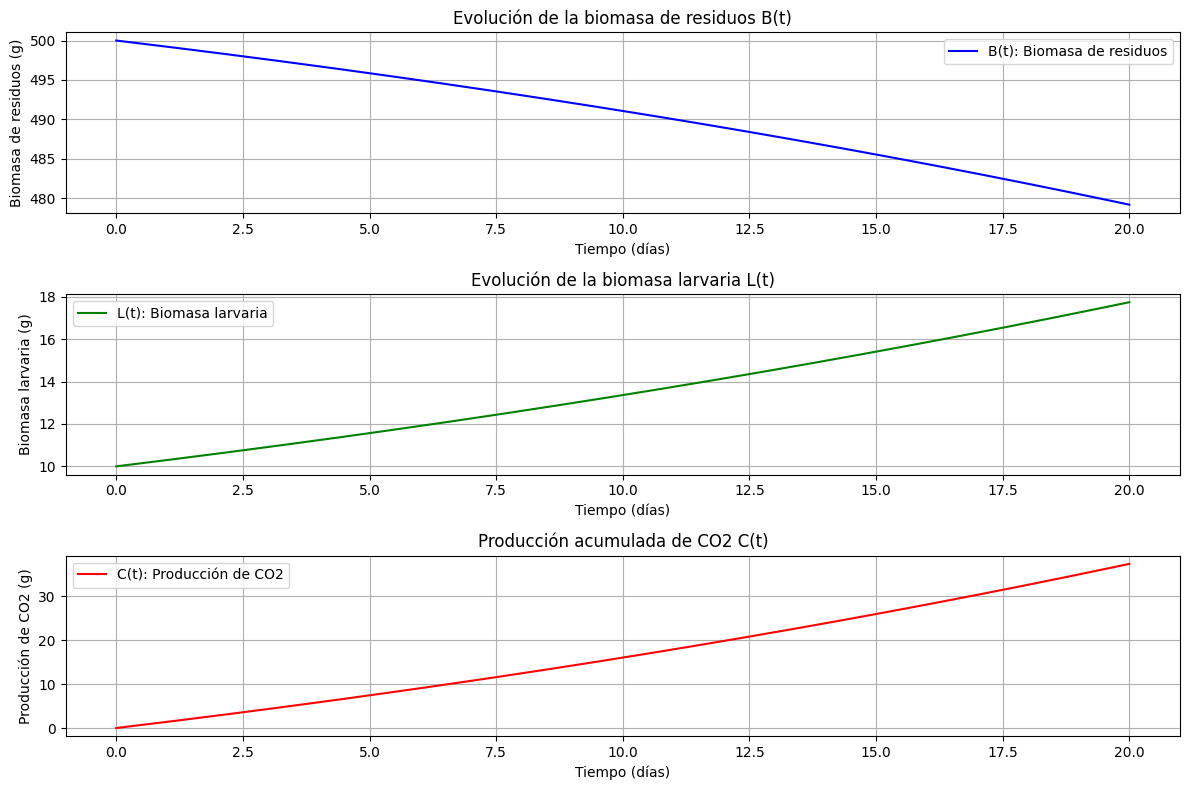
\includegraphics[width=0.8\textwidth]{solucion_ecuaciones.png} % Cambia "grafica.png" por el nombre de tu archivo
    \caption{Evolución de la biomasa de residuos ($B(t)$), biomasa larvaria ($L(t)$) y producción de $CO_2$ ($C(t)$).}
    \label{fig:resultados}
\end{figure}

Como se observa en la Figura~\ref{fig:resultados}, la biomasa de residuos disminuye con el tiempo mientras aumenta la biomasa larvaria y la producción de $CO_2$.


\section{Introducción}
El proceso de bioconversión de residuos orgánicos mediante larvas de la mosca soldado negra (\textit{Hermetia illucens}, BSFL) genera CO$_2$ como subproducto de la respiración larvaria, la actividad microbiana y la biodegradación aeróbica y anaeróbica de la materia orgánica. Este modelo matemático permite predecir la cantidad de CO$_2$ generada en función de la cantidad inicial de huevos depositados sobre un sustrato, considerando la dinámica de crecimiento larvario y las interacciones ambientales, especialmente la humedad y la temperatura.

\section{Variables y Parámetros del Modelo}
\subsection{Variables dependientes del tiempo $t$}
\begin{itemize}
    \item $N(t)$: Número de larvas en el sistema.
    \item $X(t)$ [g]: Biomasa larval.
    \item $S(t)$ [g]: Biomasa de residuos disponibles.
    \item $C(t)$ [g]: Cantidad acumulada de CO$_2$ producido.
    \item $H_s(t)$ [%]: Humedad de la biomasa.
    \item $H_a(t)$ [%]: Humedad del ambiente.
    \item $O_2(t)$ [%]: Concentración de oxígeno en el sistema.
\end{itemize}

\subsection{Parámetros constantes}
\begin{itemize}
    \item $\mu_{\max}$ [1/día]: Tasa máxima de crecimiento larval.
    \item $K_s$ [g]: Constante de semi-saturación del sustrato (Monod).
    \item $Y_{X/S}$ [g larva/g residuo]: Rendimiento de conversión de sustrato en biomasa larvaria.
    \item $Y_{C/S}$ [g CO$_2$/g residuo]: Rendimiento de CO$_2$ por unidad de residuo consumido.
    \item $\lambda_H$ [1/día]: Coeficiente de transferencia de humedad entre la biomasa y el ambiente.
    \item $k_O$ [1/día]: Tasa de consumo de oxígeno por unidad de biomasa larvaria.
    \item $E_H$ [1/día]: Tasa de evaporación de humedad desde la biomasa.
\end{itemize}

\section{Ecuaciones del Modelo}
\subsection{Dinámica de Población Larval}
\begin{equation}
    N(t) = \eta N_0 e^{-\delta t}
\end{equation}

donde $\eta$ es la tasa de eclosión y $\delta$ es la tasa de mortalidad larval.

\subsection{Crecimiento Larvario}
\begin{equation}
    \frac{dX}{dt} = Y_{X/S} \frac{\mu_{\max} S}{K_s + S} X \left( 1 - \frac{X}{X_{\max}} \right) - \delta X
\end{equation}

donde $X_{\max}$ es la biomasa larvaria máxima sostenible.

\subsection{Consumo de Residuos}
\begin{equation}
    \frac{dS}{dt} = -\frac{\mu_{\max} S}{K_s + S} X - k_s S
\end{equation}

donde $k_s$ representa la degradación espontánea del sustrato no consumido.

\subsection{Producción de CO$_2$}
\begin{equation}
    \frac{dC}{dt} = Y_{C/S} \frac{\mu_{\max} S}{K_s + S} X + k_M S \frac{O_2}{K_O + O_2}
\end{equation}

donde $k_M$ es la tasa de producción de CO$_2$ por metabolismo microbiano y $K_O$ es la constante de semi-saturación de oxígeno.

\subsection{Dinámica de Humedad y Oxígeno}
\begin{equation}
    \frac{dH_s}{dt} = -\lambda_H (H_s - H_a) - E_H H_s
\end{equation}

\begin{equation}
    \frac{dH_a}{dt} = \lambda_H (H_s - H_a)
\end{equation}

\begin{equation}
    \frac{dO_2}{dt} = -k_O X - k_M S \frac{O_2}{K_O + O_2}
\end{equation}

donde el oxígeno es consumido tanto por las larvas como por los microorganismos presentes en la biodegradación aeróbica.

\section{Interpretación del Modelo y Aplicaciones}
Este modelo matemático permite:
\begin{itemize}
    \item Predecir la producción de CO$_2$ en función de la cantidad inicial de huevos y la biomasa de sustrato.
    \item Analizar la influencia de la humedad en la eficiencia del proceso.
    \item Optimizar el diseño de biorreactores y sistemas de cultivo, ajustando condiciones ambientales para maximizar la conversión de residuos y minimizar la emisión de gases de efecto invernadero.
\end{itemize}

\section{Conclusiones}
Este modelo permite predecir la dinámica del proceso de bioconversión, incluyendo la producción de $CO_2$. Puede utilizarse para optimizar el diseño de sistemas de bioconversión y evaluar su impacto ambiental.

%\section{Referencias}
\printbibliography

\end{document}
